% !TEX root = ../thesis-sample.tex

\chapter{Isolated silver nanoparticle} \label{chap:iso_silver_np}
\graphicspath{{iso_silver_np/figs/}}

{\color{red}
Write paragraph here to introduce section, once results of the 
section are written
}

\section{Verification of \pygbe} \label{sec:verification}

In this section we show a verification study. We compare the numerical solution
obtained we \pygbe against an analytical solution available for spherical 
nanoparticles. 

The first analytical solution of the extinction cross section of spherical 
nanoparticles in vacuum, known as Mie-Theory, was presented by Gustav Mie in 1908
\cite{Mie1908}. This exact solution uses full electromagnetic theory, but in the 
long wavelength limit, electrostatics will lead us to the same solution 
\cite{BohrenHuffman1983} which is:

\begin{equation} \label{eq:Cext_analytical}
    C_\text{ext} = 4\pi a^3 k \operatorname{Im}\left(\frac{\epsilon_p/\epsilon_m -1}{\epsilon_p/\epsilon_m -2}\right)
\end{equation}

\noindent where $a$ is the radius of the nanosphere, $k$ the wave number, 
$\epsilon_p$ the dielectric constant od the nanoparticle, and $\epsilon_m$ the
dielectric constant of the host medium, in this case,  vacuum permittivity
($\epsilon_m = \epsilon_0$).  This formula, does not count for losses in the medium.
However, in 2007 Mishchenko presented a solution that counts for losses in
the host environment:

\begin{equation} \label{eq:Cext_analytical_lossy}
    C_\text{ext} = \frac{4\pi a^3}{k^\prime} \operatorname{Im}\left(k^2 \frac{\epsilon_p/\epsilon_m -1}{\epsilon_p/\epsilon_m -2}\right)
\end{equation}

\noindent where $k=k^\prime + k^{\prime\prime}i$. When the host medium is 
non-absorbing, $k$ is real ($k^{\prime\prime} = 0$ and $k=k^\prime$) and we 
recover \eqref{eq:Cext_analytical}. 

In the quasistatic limit (long wavelength approximation) the scattering 
of small particles can be explained using electrostatics, and model as
a nanosphere under a constant electric field (Figure \ref{fig:sph_field}) 
with analytical solution given by Eq. \eqref{eq:Cext_analytical_lossy}.

\begin{figure}%[h] %  figure placement: here, top, bottom, or page
    \centering
    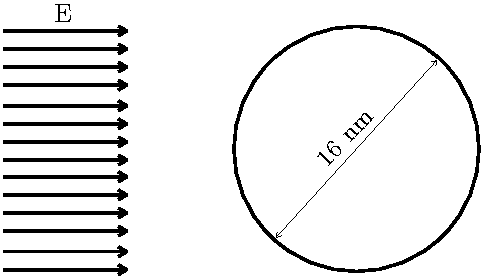
\includegraphics[width=0.55\textwidth]{sphere_field_8nm.pdf} 
    \caption{Spherical nanoparticle in a constant electric field.}
    \label{fig:sph_field}
\end{figure}

\subsection{Grid convergence analysis}\label{sub_sec:grid_conv_iso}

We perform a grid convergence analysis of \pygbe for a silver nanosphere 
of radius $r=8\,nm$ immersed in water, under a z-polarized electric field
of wavelength 380 nm and intensity of $-0.0037 e/(\text{\AA}^2 \, \epsilon_0)$.
For these conditions, the dielectric constant of water is
$1.7972 \, + \, 8.5048^{-09}i$ \cite{HaleQuerry1972} and for silver is
$-3.3877 \, + \, 0.1922i$ \cite{JohnsonChristy1972}. 
Table  \ref{table:quadparams1} shows the Gauss quadrature points used for each 
type of boundary element. We used a threshold parameter to define the near-singular
region of 0.5. This threshold defines the region of near singularity where 
semi-analytical technique is used. If $\sqrt{(2*Area)}/r > \text{threshold}$,
integration is done semi-analytically.
Table \ref{table:treeparams1} lists the parameters for the treecode and solver 
used in this convergence study.

\begin{table}%[h]
    \centering
    \caption{\label{table:quadparams1} Grid-convergence study: Gauss quadrature points; 
    $K$ and $K_{fine}$ are per element; $N_k $ is per element edge (semi-analytical integration). } 
    \begin{tabular}{l l}
    \hline%\toprule
     distant elements: & $K=4$ \\
     near-singular integrals:   & $ K_{fine}=37$ \\
     singular elements:  & $N_k =9$ \\
    \hline%\bottomrule
    \end{tabular}
\end{table}


\begin{table}%[h]
    \centering
    \caption{\label{table:treeparams1} Grid-convergence study: treecode and solver parameters.} 
    \begin{tabular}{l l}
    \hline%\toprule
    treecode order of expansion: & $P=15$\\
    MAC                          & $\theta=0.5$\\
    GMRES tolerance                    & $10^{-5}$\\
    \hline%\bottomrule
    \end{tabular}
\end{table}

Figure \ref{fig:conv_iso_sph} shows the results for the convergence study, with meshes of sizes 512, 2048, 
8192 and 32768 elements. The errors (Table \ref{table:err_iso_sph}) are computed against 
the analytical solution $C_{ext} = 1854.48$ nm$^2$ computed using Equation \eqref{eq:Cext_analytical_lossy}.
The dash line in Figure \ref{fig:conv_iso_sph} corresponds to a $1/N$ slope, and the observed order of 
convergence is $0.98$ which indicates that the meshes are correctly resolving the numerical solution with \pygbe.
The $1/N$ rate of convergence is consistent with convergence results in
previous work using \pygbe \cite{CooperBardhanBarba2013}. 

\begin{figure}[h] %  figure placement: here, top, bottom, or page
    \centering
    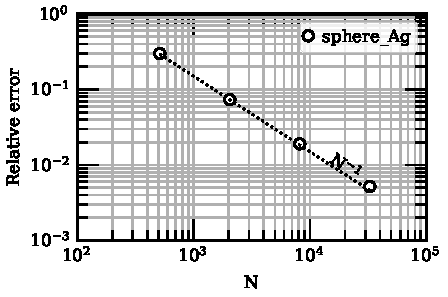
\includegraphics[width=0.65\textwidth]{convergence_sph_Ag_R8_w380.pdf} 
    \caption{Grid-convergence study for the extinction cross-section of a spherical silver
             nanoparticle, computed with \pygbe. Figure, plotting script and auxiliary files 
             available under \textsc{cc-by} \cite{ClementiETal2018c}.}
    \label{fig:conv_iso_sph}
 \end{figure}
 
 
 \begin{table}[h]
     \centering
     \caption{\label{table:err_iso_sph} Percentage error in the grid-convergence cases with an 
     isolated silver nanosphere.} 
     \begin{tabular}{c c}
     \hline%\toprule
     N & \% error \\
     \hline%\midrule
      $512$ & $29.86$ \\
      $2048$ & $7.33$ \\
      $8192$ & $1.9$ \\
      $32768$ & $0.52$ \\
     \hline%\bottomrule
     \end{tabular}
 \end{table}


\subsection{LSPR response of silver nanosphere}\label{sub_sec:lspr_silver_np}

To complement the verification test for the Localized Surface Plasmon Resonance (LSPR) implementation
on \pygbe, we computed the extinction cross section of the isolated silver sphere across multiple 
wavelengths. Figure \ref{fig:verif_sph} shows the results of comparing the simulations with the
analytical solution for a range of wavelengths from $[370-400]$ nm. The values of the dielectric 
for each wavelength were obtained by interpolation of experimental data 
\cite{HaleQuerry1972, JohnsonChristy1972}. To reproduce the interpolation study, we create
a Jupyter notebook and supporting code that can be find as part of the execution files
repro-package \cite{ClementiETal2018b}.
For this verification exercise we use a mesh of $N=32768$, and we relaxed some parameters 
compared to the ones used in the convergence analysis from section \ref{sub_sec:grid_conv_iso} 
that are shown in Tables \ref{table:quadparams2} and \ref{table:treeparams2}. The errors for each 
frequency are below $1\%$, and each runtime decrease by $12\times$.
Figure \ref{fig:verif_sph} exposes a good agreement between the analytical and simulation results, 
showing that \pygbe can accurately represent the mathematical model. Moreover, we can say that 
the level of accuracy is sufficient, given that the experimental uncertainty for the dielectric 
values for silver is in the order of $1\%$ \cite{JohnsonChristy1972}. 

\begin{figure}%[h] %  figure placement: here, top, bottom, or page
    \centering
    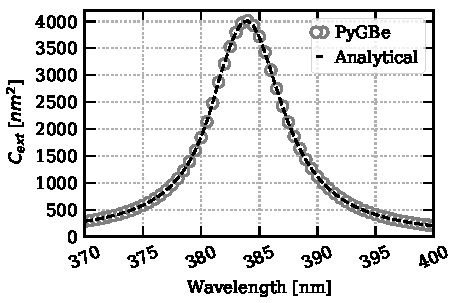
\includegraphics[width=0.65\textwidth]{silver_NP_verification.pdf} 
    \caption{Extinction cross-section as a function of wavelength for an $8$ nm
             silver sphere immersed in water. The peak in the values of 
             extinction cross-section corresponds to the plasmon resonance of the metallic 
             nanoparticle under the incoming electric field. Figure, plotting script and 
             auxiliary files available under \textsc{cc-by} \cite{ClementiETal2018d}.}
    \label{fig:verif_sph}
 \end{figure}

\begin{table}%[h]
    \centering
    \caption{\label{table:quadparams2} Verification: Gauss quadrature points; 
    $K$ and $K_{fine}$ are per element; $N_k $ is per element edge (semi-analytical integration). } 
    \begin{tabular}{l l}
    \hline%\toprule
     distant elements: & $K=4$ \\
     near-singular integrals:   & $ K_{fine}=19$ \\
     singular elements:  & $N_k =9$ \\
    \hline%\bottomrule
    \end{tabular}
\end{table}


\begin{table}%[h]
    \centering
    \caption{\label{table:treeparams2} Verification: treecode and solver parameters.} 
    \begin{tabular}{l l}
    \hline%\toprule
    treecode order of expansion: & $P=6$\\
    MAC                                         & $\theta=0.5$\\
    GMRES tolerance                    & $10^{-3}$\\
    \hline%\bottomrule
    \end{tabular}
\end{table}
